\documentclass{ximera}

\input{../../preamble.tex}

\author{Bobby Ramsey}

\outcome{Add up a large number of terms quickly using sigma notation.}
\outcome{Compute left, right, and midpoint Riemann Sums with many rectangles.}
\outcome{Understand the relationship between area under a curve and sums of rectangles.}
\outcome{Approximate area under a curve.}
\outcome{Understand how the area under a curve is related to the antiderivative.}
\outcome{Use limits of Riemann sums to find the exact area under a curve.}
\outcome{Understand how Riemann sums are used to find exact area.}

\begin{document}

\begin{exercise}
Let $f(x) = x^2-1$. 
		\begin{image}
			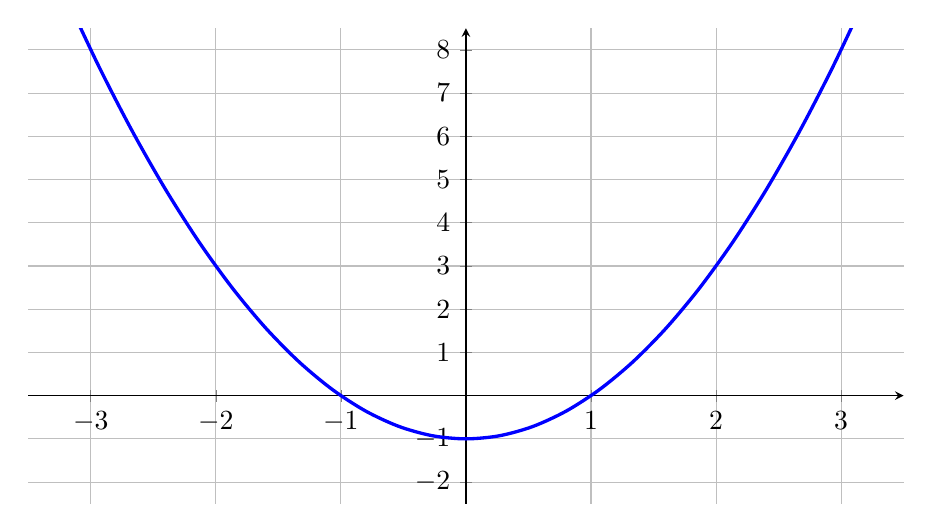
\begin{tikzpicture}
					\begin{axis}[
						xmin=-3.5, xmax=3.5, ymin=-2.5,ymax=8.5,    
						axis lines =middle, 
						every axis y label/.style={at=(current axis.above origin),anchor=south},
						every axis x label/.style={at=(current axis.right of origin),anchor=west},
						xtick={-3,...,3}, ytick={-2,...,8},
						grid=major, width=5in, height=3in,
						]
						\addplot[color=blue, very thick, smooth, domain=-3.2:3.2]{x^2-1};	
					\end{axis}
			\end{tikzpicture}
		\end{image}

	We are calculating the value of $\displaystyle \int_{-1}^{2} f(x) \d x$.



	We start by setting up the Riemann sum using $n$ rectangles using right endpoints.
	What is $\Delta x$?
	
	\[ \Delta x = \answer{3/n} \]
	\begin{hint}
		Remember that $\Delta x = \frac{b-a}{n}$
	\end{hint}
	\begin{exercise}
		Which of the following gives our choice of sample points?
		\begin{multipleChoice}
			\choice[correct]{$x_k^* = -1 + \frac{3k}{n}$}
			\choice{$x_k^* = -1 + \frac{3(k-1)}{n}$}
			\choice{$x_k^* = -1 + \frac{3\left(k-\frac{1}{2}\right)}{n}$}
		\end{multipleChoice}
		\begin{hint}
			Are we using for our sample points?
		\end{hint}
		\begin{exercise}
			Calculate $f(x_k^*) \Delta x$ in terms of $k$ and $n$.
			
			\[ f(x_k^*) \Delta x = \frac{\answer{27}k^2}{n^3}-\frac{\answer{18}k}{n^2} \]
			\begin{hint}
				You've found $x_k^*$.  Plug it into the formula for $f$ above and multiply by $\Delta x$.
				Your answer will have $k$'s and $n$'s in it, but no $x$'s.
			\end{hint}
			\begin{exercise}
				Using $f(x_k^*)\Delta x = \frac{27}{n^3}k^2 - \frac{18}{n^2}k$ (which you found above), evaluate the Riemann sum.  (It will be in terms of $n$).
				
				\begin{align*}
					\sum_{k=1}^{n} f(x_k^*)\Delta x &=  \sum_{k=1}^{n} \left(\frac{27}{n^3}\answer{k^2} + \frac{18}{n^2}\answer{k}\right)\\
						&= \frac{27}{n^3} \sum_{k=1}^{n} \answer{k^2} + \frac{18}{n^2} \sum_{k=1}^{n} \answer{k}\\
						&= \frac{27}{n^3} \left( \answer{\frac{n(n+1)(2n+1)}{6}}\right) + \frac{18}{n^2} \left( \answer{\frac{n(n+1)}{2}}\right)\\
						&= \answer{\frac{9(n+1)(2n+1)}{2n^2}-\frac{9(n+1)}{n}}
				\end{align*}
				
				\begin{exercise}
					Using what you've found for the Riemann sum, evaluate the definite integral by taking the limit.
					\[ \int_{-1}^{2} (x^2-1) \d x = \lim_{n\to\infty} \sum_{k=1}^{n} f(x_k^*)\Delta x = \answer{0} \]
				\end{exercise}
			\end{exercise}
		\end{exercise}
	\end{exercise}
\end{exercise}

\end{document}
